The implementation of the breast cancer detection system was conducted in two parts. The first part corresponds to a common pipeline developed in group, and the second part to individual implementations using the common pipeline as a baseline. The distribution of work during the implementation of the common pipeline can be found in Appendix~\ref{ch:appendix-team-meeting-summaries}.

\begin{figure}[ht]
\centerline{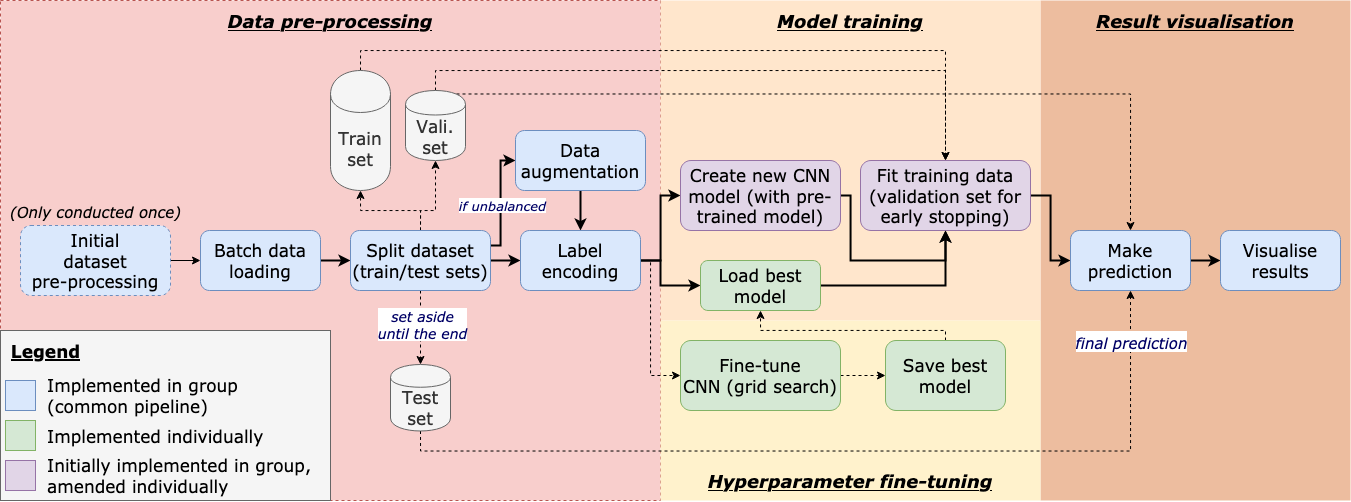
\includegraphics[width=1.25\textwidth]{Dissertation/figures/implementation/detailed flowchart.png}}
\caption{\label{fig:implementation-detailed-flowchart}Flowchart. Created using draw.io.}
\end{figure}

%%%%%%%%%%%%%%%%%%%%%%%%%%%%%%%%%%%%%%%%%%%%%


\section{Implementation of common deep learning pipeline}

%%%%%%%%%%%%%%%

\subsection{Data pre-processing}

\subsubsection{Processing and organising raw images}

Two scripts written to read CSV files and reorganise the images in folders for classification.\\

File formats: PGM and DICOM files need to be converted.\\

Scikit-Learn's label encoder to one-hot encode labels.


\subsubsection{Data loading}

TF cache and batch functions.\\

Image resizing to fit in pre-trained CNN models (e.g. VGG19 model needs 224x224px image size).\\

Normalising images to fit in [0-1] float range rather than [0-255] integer range.

%%%%%%%%%%%%%%%%%%%%%%%%%%%%%%%%%%%%%%%%%%%%%

\subsection{CNN Model}

Once the CNN model is finished training model is saved in HDF5 format in order to save the model's architecture, the layers' hyperparameters, all the connection weights and biases that were learned during training \cite{Geron2019} and the optimiser used.\\

Train test split is already done for CBIS-DDSM dataset.

%%%%%%%%%%%%%%%%%%%%%%%%%%%%%%%%%%%%%%%%%%%%%

\subsection{Output}

todo
